\subsection{Small loop antenna}

\begin{frame}{Small loop antenna}
    \begin{columns}
        \column{0.5\textwidth}
        \begin{align*}
            \mathbf{A} &= \dfrac{\mu l_1 I}{4 \pi} \left[ \dfrac{\exp ( - j \beta r_1 )}{r_1} - \dfrac{\exp ( - j \beta r_3 )}{r_3} \right] \mathbf{\hat{x}} \\
            &+ \dfrac{\mu l_2 I}{4 \pi} \left[ \dfrac{\exp ( - j \beta r_2 )}{r_2} - \dfrac{\exp ( - j \beta r_4 )}{r_4} \right] \mathbf{\hat{y}} \\
            & \approx j \beta S \dfrac{\mu I}{4\pi} \dfrac{\exp ( - j \beta r )}{r} \sin \theta \mathbf{\hat{\phi}}.
        \end{align*}
        
        \vspace{3mm}
        Note: \( r_1-r_3 = \Delta r_{13} \approx l_2 \cos \theta \ll r_i \)
        \begin{align*}
            \Rightarrow f(r_1) - f(r_3) &= f'(r) \cdot \Delta r_{13}. \\
            &= \nabla f(r) \cdot \Delta \mathbf{r}_{13}.
        \end{align*}
        \column{0.5\textwidth}
        \vspace{-8mm}
        \begin{figure}
            \centering
            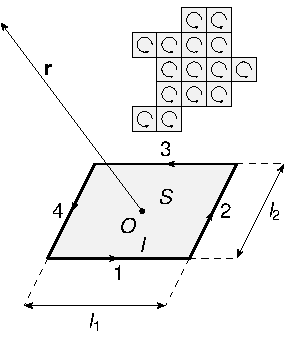
\includegraphics[width=\textwidth]{Figures/Small_loop.pdf}
            \caption{Rectangle small loop antenna.}
            \label{fig:small_loop}
        \end{figure}
    \end{columns}
\end{frame}